% Original schematic of the implemented THERA-Net workflow.
% Compile here: pdflatex -interaction=nonstopmode -halt-on-error thera_framework.tex
% Natural size: 6.5 inches wide. Include without resizing to preserve 14 TeX pt.
\documentclass[border=0pt]{standalone}
\usepackage[T1]{fontenc}
\usepackage{lmodern,amsmath,amssymb,bm,tikz}
\usetikzlibrary{arrows.meta,calc}
\DeclareMathSizes{14}{14}{10}{7}
\definecolor{neural}{HTML}{28618C}
\definecolor{neuralfill}{HTML}{EFF5FA}
\definecolor{physical}{HTML}{32746B}
\definecolor{physicalfill}{HTML}{EDF5F1}
\definecolor{losscolor}{HTML}{996B25}
\definecolor{lossfill}{HTML}{FBF4E7}
\definecolor{backprop}{HTML}{AE4C4B}
\definecolor{ink}{HTML}{27313B}
\begin{document}
\fontsize{14}{17}\selectfont
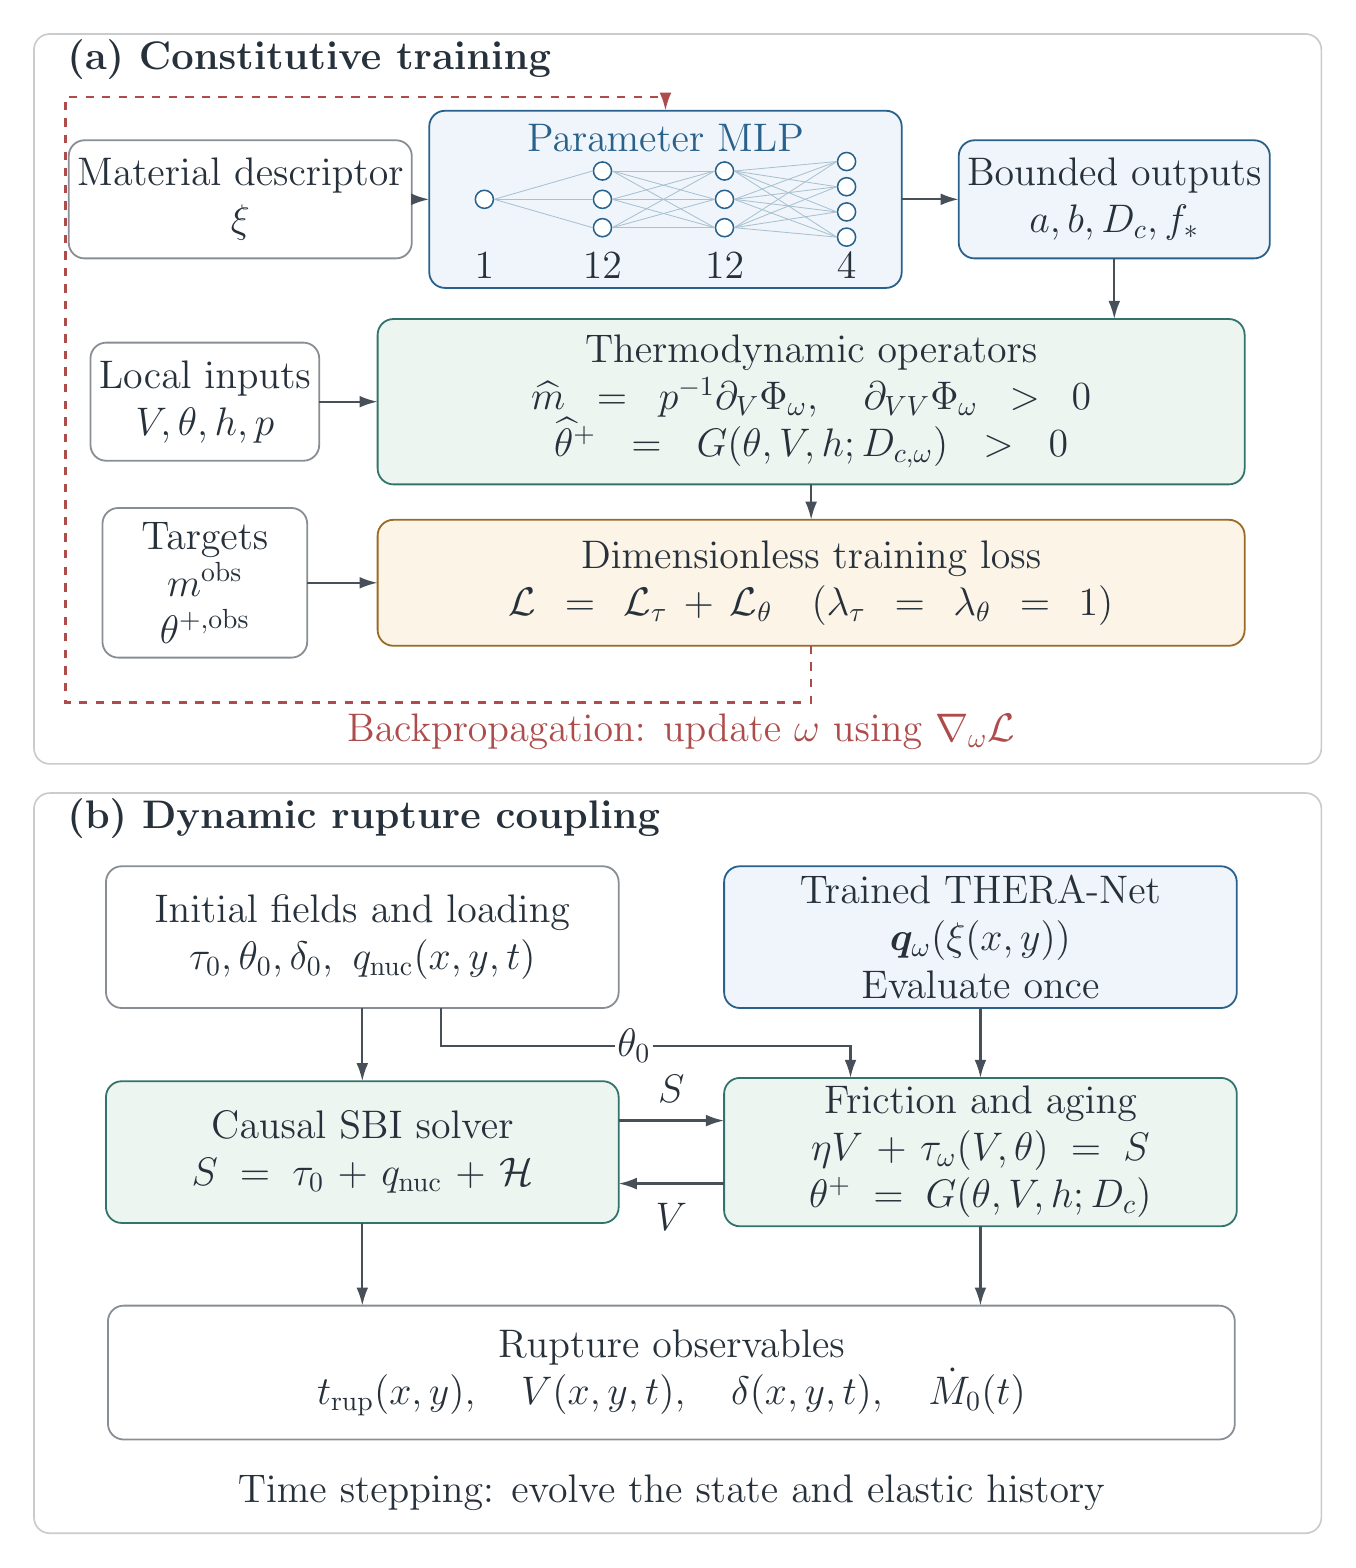
\begin{tikzpicture}[
 x=1cm,y=1cm,
 every node/.style={font=\fontsize{14}{17}\selectfont,text=ink},
 box/.style={draw=ink!55,fill=white,rounded corners=2mm,line width=.65pt,
             align=center,inner sep=3pt,outer sep=0pt},
 nn/.style={box,draw=neural,fill=neuralfill},
 phys/.style={box,draw=physical,fill=physicalfill},
 loss/.style={box,draw=losscolor,fill=lossfill},
 flow/.style={-{Latex[length=2.3mm,width=1.5mm]},line width=.8pt,draw=ink!85},
 grad/.style={flow,draw=backprop,dashed,line width=.9pt},
 neuron/.style={circle,draw=neural,fill=white,inner sep=0pt,minimum size=2.3mm,line width=.55pt}
]
\path[use as bounding box] (0,0) rectangle (16.51,-19.2);
\draw[rounded corners=2mm,draw=ink!25,line width=.6pt]
  (.08,-.08) rectangle (16.43,-9.35);
\draw[rounded corners=2mm,draw=ink!25,line width=.6pt]
  (.08,-9.72) rectangle (16.43,-19.12);

% (a) Offline constitutive learning. The network input is xi alone.
\node[anchor=west,font=\bfseries\fontsize{14}{17}\selectfont]
  at (.38,-.40) {(a) Constitutive training};
\node[box,minimum width=3.3cm,minimum height=1.5cm] (descriptor)
  at (2.70,-2.18) {Material descriptor\\$\xi$};
\node[nn,minimum width=6cm,minimum height=2.25cm] (network)
  at (8.10,-2.18) {};
\node[text=neural] at (8.10,-1.40) {Parameter MLP};
\node[neuron] (n00) at (5.80,-2.18) {};
\foreach \j/\yy in {1/-1.82,2/-2.18,3/-2.54}{
  \node[neuron] (n1\j) at (7.30,\yy) {};
  \node[neuron] (n2\j) at (8.85,\yy) {};
}
\foreach \j/\yy in {1/-1.70,2/-2.02,3/-2.34,4/-2.66}{
  \node[neuron] (n3\j) at (10.40,\yy) {};
}
\foreach \j in {1,2,3}{
  \draw[neural!40,line width=.3pt] (n00.east)--(n1\j.west);
  \foreach \k in {1,2,3}{\draw[neural!40,line width=.3pt] (n1\j.east)--(n2\k.west);}
  \foreach \k in {1,2,3,4}{\draw[neural!40,line width=.3pt] (n2\j.east)--(n3\k.west);}
}
\foreach \xx/\count in {5.80/1,7.30/12,8.85/12,10.40/4}{
  \node at (\xx,-3.02) {$\count$};
}
\node[nn,minimum width=3.5cm,minimum height=1.5cm] (parameters)
  at (13.80,-2.18) {Bounded outputs\\$a,b,D_c,f_*$};
\draw[flow] (descriptor.east)--(network.west);
\draw[flow] (network.east)--(parameters.west);

\node[box,minimum width=2.6cm,minimum height=1.5cm] (local)
  at (2.25,-4.75) {Local inputs\\$V,\theta,h,p$};
\node[phys,text width=10.8cm,minimum height=2.1cm] (operators)
  at (9.95,-4.75) {Thermodynamic operators\\
  $\widehat m=p^{-1}\partial_V\Phi_\omega,\quad\partial_{VV}\Phi_\omega>0$\\
  $\widehat\theta^+=G(\theta,V,h;D_{c,\omega})>0$};
\draw[flow] (local.east)--(operators.west);
\draw[flow] (parameters.south)--(parameters.south |- operators.north);

\node[box,minimum width=2.6cm,minimum height=1.9cm] (targets)
  at (2.25,-7.05) {Targets\\$m^{\mathrm{obs}}$\\$\theta^{+,\mathrm{obs}}$};
\node[loss,text width=10.8cm,minimum height=1.6cm] (objective)
  at (9.95,-7.05) {Dimensionless training loss\\
  $\mathcal L=\mathcal L_\tau+\mathcal L_\theta\quad
   (\lambda_\tau=\lambda_\theta=1)$};
\draw[flow] (operators.south)--(objective.north);
\draw[flow] (targets.east)--(objective.west);
\draw[grad] (objective.south)--(9.95,-8.57)--(.48,-8.57)
  --(.48,-.88)--(8.10,-.88)--(network.north);
\node[text=backprop] at (8.30,-8.94)
  {Backpropagation: update $\omega$ using $\nabla_\omega\mathcal L$};

% (b) Online deployment. Fixed parameters are evaluated once; only the
% physical state and causal elastic history are evolved by the solver.
\node[anchor=west,font=\bfseries\fontsize{14}{17}\selectfont]
  at (.38,-10.05) {(b) Dynamic rupture coupling};
\node[box,text width=6.3cm,minimum height=1.8cm] (initial)
  at (4.25,-11.55) {Initial fields and loading\\
  $\tau_0,\theta_0,\delta_0,\ q_{\mathrm{nuc}}(x,y,t)$};
\node[nn,text width=6.3cm,minimum height=1.8cm] (frozen)
  at (12.10,-11.55) {Trained THERA-Net\\
  $\bm q_\omega(\xi(x,y))$\\Evaluate once};
\node[phys,text width=6.3cm,minimum height=1.8cm] (sbi)
  at (4.25,-14.28) {Causal SBI solver\\
  $S=\tau_0+q_{\mathrm{nuc}}+\mathcal H$};
\node[phys,text width=6.3cm,minimum height=1.8cm] (friction)
  at (12.10,-14.28) {Friction and aging\\
  $\eta V+\tau_\omega(V,\theta)=S$\\
  $\theta^+=G(\theta,V,h;D_c)$};
\draw[flow] (initial.south)--(sbi.north);
\draw[flow] (frozen.south)--(friction.north);
\coordinate (stateentry) at (10.45,-12.93);
\draw[flow] ($(initial.south)+(1,0)$)--(5.25,-12.93)
  --(stateentry)--(stateentry |- friction.north);
\node[fill=white,inner sep=1pt] at (7.70,-12.93) {$\theta_0$};
\draw[flow] ($(sbi.east)+(0,.40)$)--($(friction.west)+(0,.40)$);
\node[fill=white,inner sep=.5pt] at (8.175,-13.48) {$S$};
\draw[flow] ($(friction.west)+(0,-.40)$)--($(sbi.east)+(0,-.40)$);
\node[fill=white,inner sep=.5pt] at (8.175,-15.10) {$V$};
\node[box,text width=14.1cm,minimum height=1.7cm] (outputs)
  at (8.175,-17.08) {Rupture observables\\
  $t_{\mathrm{rup}}(x,y),\quad V(x,y,t),\quad
   \delta(x,y,t),\quad\dot M_0(t)$};
\draw[flow] (sbi.south)--(sbi.south |- outputs.north);
\draw[flow] (friction.south)--(friction.south |- outputs.north);
\node at (8.175,-18.60) {Time stepping: evolve the state and elastic history};
\end{tikzpicture}
\end{document}
